\documentclass[tikz,border=0pt,11pt]{standalone}
\usepackage[T1]{fontenc}
\usepackage[utf8]{inputenc}
\usepackage{lmodern,amsmath,amssymb}
\usepackage[swedish]{babel}
\usetikzlibrary{arrows.meta,calc,positioning,decorations.pathmorphing,decorations.pathreplacing,patterns,shadings}
\definecolor{navy}{HTML}{102F40}
\definecolor{teal}{HTML}{147D78}
\definecolor{lightteal}{HTML}{E6F1ED}
\definecolor{gold}{HTML}{B88B3B}
\definecolor{palegold}{HTML}{F7EEDB}
\definecolor{rust}{HTML}{B6533B}
\definecolor{palerust}{HTML}{FAEAE4}
\definecolor{paper}{HTML}{F7F5EE}
\definecolor{muted}{HTML}{5B6D72}
\definecolor{line}{HTML}{D6DED8}
\renewcommand{\familydefault}{\sfdefault}
\newcommand{\atom}[5]{\shade[ball color=#3!70] (#1,#2) circle (#5);\node[text=white,font=\bfseries\small] at (#1,#2){#4};}
\newcommand{\water}[3]{\begin{scope}[shift={(#1,#2)},scale=#3]\draw[navy!45,line width=2pt] (-.3,.22)--(0,0)--(.3,.22);\atom{0}{0}{rust}{O}{.22}\atom{-.3}{.22}{teal}{H}{.15}\atom{.3}{.22}{teal}{H}{.15}\end{scope}}
\newcommand{\panel}[4]{\filldraw[fill=white,draw=line,rounded corners=5pt] (#1,#2) rectangle ++(#3,#4);}
\newcommand{\note}[4]{\node[txt,text width=#3cm] at (#1,#2){#4};}
\tikzset{txt/.style={anchor=north west,align=left,text=navy,font=\small},
 head/.style={anchor=west,text=navy,font=\bfseries\large},
 label/.style={align=center,text=navy,font=\small},
 smalllabel/.style={align=center,text=muted,font=\footnotesize},
 arrow/.style={-{Latex[length=2.5mm,width=1.8mm]},line width=1.2pt,draw=teal},
 goldarrow/.style={-{Latex[length=2.5mm]},line width=1.2pt,draw=gold},
 rustarrow/.style={-{Latex[length=2.5mm]},line width=1.2pt,draw=rust},
 dashedarrow/.style={arrow,dashed},
 badge/.style={fill=lightteal,rounded corners=3pt,text=teal,font=\bfseries\small,inner sep=5pt}}
\begin{document}
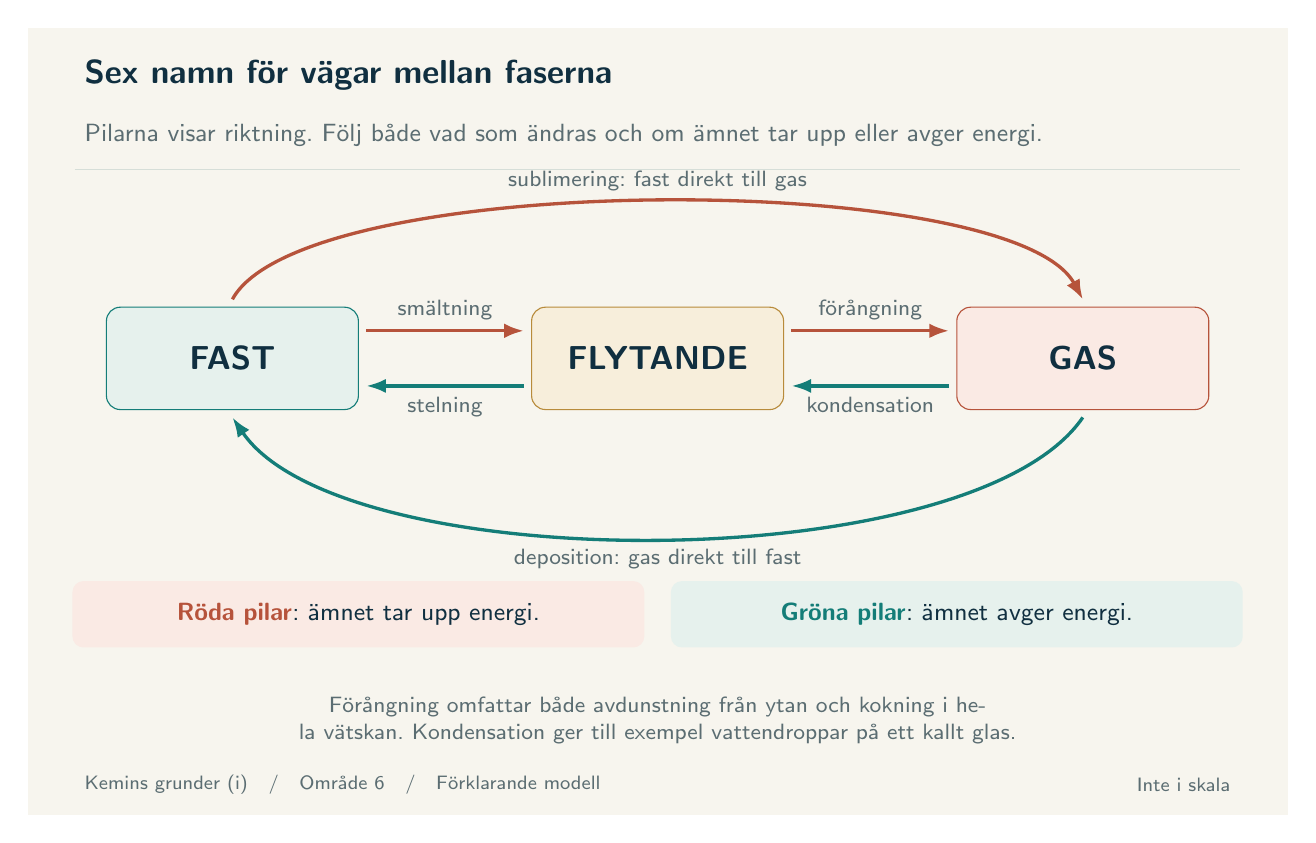
\begin{tikzpicture}[x=1cm,y=1cm]
\path[use as bounding box] (0,0) rectangle (16,10);
\fill[paper] (0,0) rectangle (16,10);
\node[head] at (.6,9.4){Sex namn för vägar mellan faserna};
\note{.6}{8.9}{14.8}{\textcolor{muted}{Pilarna visar riktning. Följ både vad som ändras och om ämnet tar upp eller avger energi.}}
\draw[line] (.6,8.2)--(15.4,8.2);

\node[fill=lightteal,draw=teal,rounded corners=5pt,minimum width=3.2cm,minimum height=1.3cm,font=\bfseries\large,text=navy] (solid) at (2.6,5.8){FAST};
\node[fill=palegold,draw=gold,rounded corners=5pt,minimum width=3.2cm,minimum height=1.3cm,font=\bfseries\large,text=navy] (liquid) at (8,5.8){FLYTANDE};
\node[fill=palerust,draw=rust,rounded corners=5pt,minimum width=3.2cm,minimum height=1.3cm,font=\bfseries\large,text=navy] (gas) at (13.4,5.8){GAS};
;
\draw[rustarrow] (4.3,6.15)--(6.3,6.15) node[midway,above,smalllabel]{smältning};
\draw[arrow] (6.3,5.45)--(4.3,5.45) node[midway,below,smalllabel]{stelning};
\draw[rustarrow] (9.7,6.15)--(11.7,6.15) node[midway,above,smalllabel]{förångning};
\draw[arrow] (11.7,5.45)--(9.7,5.45) node[midway,below,smalllabel]{kondensation};
\draw[rustarrow] (2.6,6.55)..controls(3.5,8.2)and(12.5,8.2)..(13.4,6.55) node[midway,above,smalllabel]{sublimering: fast direkt till gas};
\draw[arrow] (13.4,5.05)..controls(12,3)and(4,3)..(2.6,5.05) node[midway,below,smalllabel]{deposition: gas direkt till fast};
\node[label,text width=6.7cm,fill=palerust,rounded corners=4pt,inner sep=8pt] at (4.2,2.55){\textcolor{rust}{\textbf{Röda pilar}}: ämnet tar upp energi.};
\node[label,text width=6.7cm,fill=lightteal,rounded corners=4pt,inner sep=8pt] at (11.8,2.55){\textcolor{teal}{\textbf{Gröna pilar}}: ämnet avger energi.};
\node[smalllabel,text width=14cm] at (8,1.2){Förångning omfattar både avdunstning från ytan och kokning i hela vätskan. Kondensation ger till exempel vattendroppar på ett kallt glas.};\node[anchor=west,text=muted,font=\scriptsize] at (.6,.38){Kemins grunder (i)\quad /\quad Område 6\quad /\quad Förklarande modell};
\node[anchor=east,text=muted,font=\scriptsize] at (15.4,.38){Inte i skala};
\end{tikzpicture}\end{document}
